\documentclass{article}

\usepackage{tikz}
\usetikzlibrary{automata, quotes, calc, arrows.meta}
\usepackage[czech]{babel} 
\usepackage[utf8]{inputenc}
\usepackage[T1]{fontenc}
%\usepackage[IL2]{fontenc} % Different type of font for wierdos
\usepackage{graphicx} % Required for the inclusion of images
\usepackage{natbib} % Required to change bibliography style to APA
\usepackage{amsmath} % Required for some math elements 
\usepackage{amsfonts}
\usepackage{amssymb}
\usepackage{booktabs}
\usepackage{epstopdf}
\usepackage{multicol}
\usepackage{color}
\usepackage{float}
\usepackage[total={15.5cm,23.5cm}, top=2.5cm, left=3cm, includefoot]{geometry}
\usepackage[colorlinks=true,linkcolor = black, urlcolor = black, citecolor = black]{hyperref}
\usepackage{enumitem}
\usepackage{subfig}
\usepackage[toc,page]{appendix}
\usepackage{hyperref} 
\usepackage{matlab-prettifier}
\usepackage{datetime}
\usepackage{mathtools}
\usepackage[thinc]{esdiff}
\usepackage{listings}
\usepackage{xcolor} % For custom colors

\begin{document}


\begin{titlepage}

\centering

{\scshape\LARGE Západočeská univerzita\par}
{\scshape\Large Fakulta aplikovaných věd \par}
{\scshape\Large Katerdra Kybernetiky \par}
{\begin{center}
    
\includegraphics[width=0.7\textwidth]{pic/fav.jpg} 
\end{center}}

{\huge\bfseries První semestrální práce z STP \par}

\vspace{2cm}

{\Large\itshape Samuel Kokoška, Martin Hamar\par}

\vfill

\vspace{1cm}

\hskip -1 cm{KKY/STP} \hfill {Datum: \today }



\end{titlepage}

\section{Úvod}
V rámci první semestrální práce ze přemětu `Stochastické systémy a procesy' je cílem vypracovat dva příklady týkající se Markovských řetězců.
V prvním příkladu musí být řetězec regulární a homogenní a máme pro něj určit stření počet kroků, které jsou třeba k prvnímu dosažení stavu \verb|j| za předpokladu, že se vycházelo ze stavu \verb|i|. Poté máme také určit finální pravděpodobnosti.

V druhém příkladu pracujeme s homogenním řetězecem, kde jsou dva absorpční stavy. 
Zde máme určit střední počet průchodů stavem \verb|j|, pokud se vychází ze stavu \verb|i|, do té doby než dojde k pohlcení. Poté musíme vypočítat dobu pobytu v tranzientním stavu. Poslední podúkol příkladu 2 je spočtení ppst skončení v absorpčím stavu, pro všechny tranzientní stavy.
Celé zadání je k vidění v sekci~\ref{ssec:zadani}. 


Během vypracovávání byl použit Matlab pro jeho schopnost pracování s maticemi a rovnicemi. Postupy řešení pro jednotlivé příklady jsou k vidění v sekci \ref{sec:postup}.




\subsection{Zadání}\label{ssec:zadani}
\begin{figure} [htb!]
    \centering
    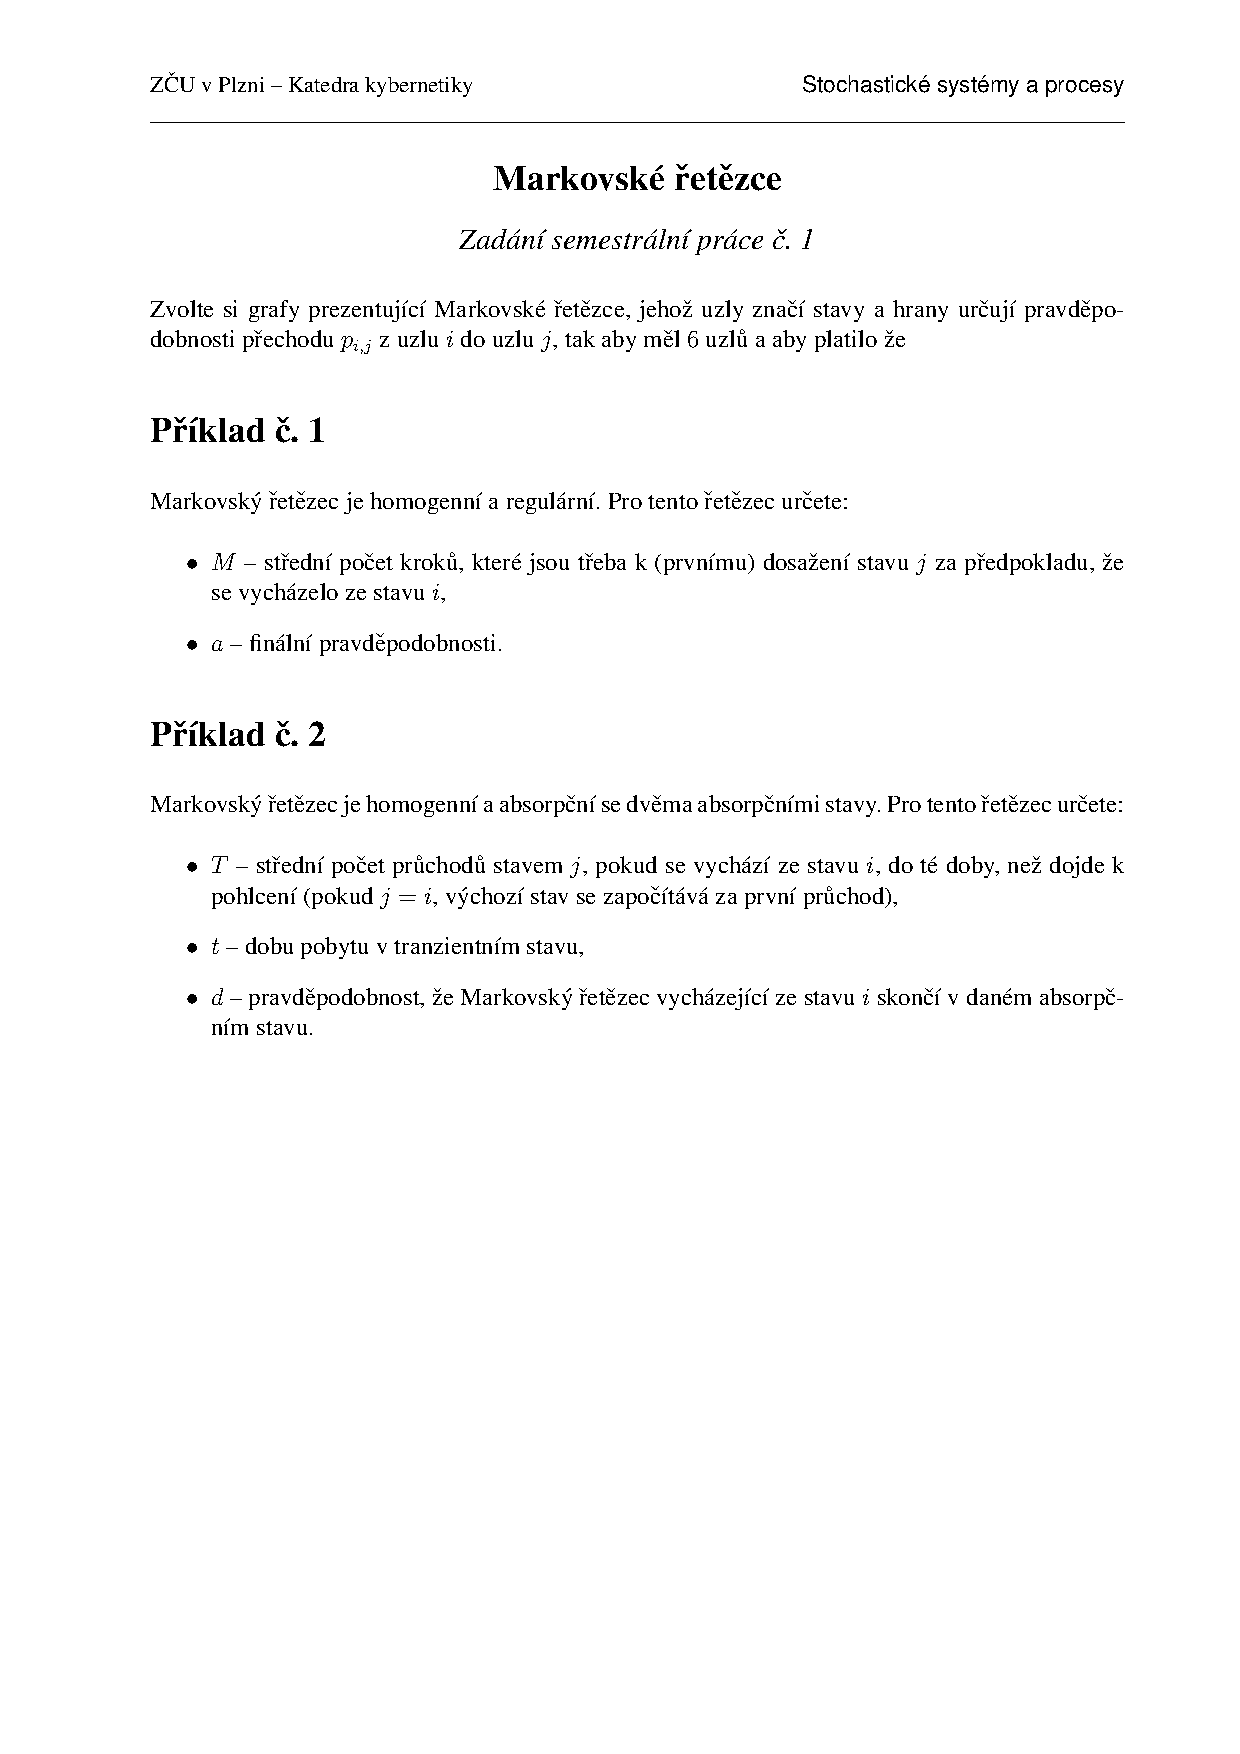
\includegraphics[width = 0.7\textwidth]{zadani.pdf}
    %\includesvg[width = 1\textwidth]{pic/XXX}
\end{figure}
\clearpage
\section{Postup Řešení}\label{sec:postup}
\subsection{Příklad 1}
Pro tento příklad by zvolen řetězec znázorněn na obrázku~\ref{fig:markov_chain_1}. Odpovídající matice $\mathbf{P}$ vypadá takto: 
\[
\mathbf{P} =
\begin{bmatrix}
0 & 0 & 1 & 0 & 0 & 0 \\
1 & 0 & 0 & 0 & 0 & 0 \\
0 & 0.5 & 0 & 0.5 & 0 & 0 \\
0 & 0 & 0.5 & 0 & 0.5 & 0 \\
0 & 0 & 0 & 0 & 0 & 1 \\
0 & 0 & 0 & 1 & 0 & 0 \\
\end{bmatrix}.
\]

Nejdříve je snažší si u tohoto příkladu spočítat finální ppsti, ty si spočítáme pomocí vztahu $\pi = \pi \mathbf{P}$, kde $\pi$ je vektor, který hledáme. Po úpravě řešíme soustavu rovnic: $(P^T - \mathbf{I})\pi^T = \mathbf{0}$, za podmínky že členy vektoru $\pi$ musí mít součet jedna.
S vyřešením této rovnice nám pomůže matlab a jejím výsledkem pro matici $\mathbf P$ sepsanou výše je:
\[
\pi = 
\begin{bmatrix}
    \frac 1 8 & \frac 1 8 & \frac 1 4 & \frac 1 4 &  \frac 1 8 & \frac 1 8 
\end{bmatrix}.
\]

Nyní si spočítáme matici $\mathbf{M}$, která určuje stření počet kroků, které jsou třeba k prvnímu dosažení stavu \verb|j| za předpokladu, že se vycházelo ze stavu \verb|i|. 
Zde na to půjdeme přes simulaci absorpčních stavů. 
Postupně uděláme z každého stavu absorpční a spočítáme pro něj fundamentální matici $\mathbf{T} = (\mathbf{I} - \mathbf{Q})$.
Z té poté spočítáme střední dobu strávenou v tranzientních stavech $t = \mathbf{T}\mathbf{1}$ - to jsou všechny ty co nejsou absorpční. 
Tento vektor poté vložíme do matice $\mathbf{M}$, na místo určené vybraným absorpčním stavem. 

Je důležité podotknout, že tímto postupem získáme na diagonále nulové prvky, protože tímto výpočtem vždy považujeme prvek za absorpční a nemá smysl pro něj spočítat první dosažení.
Tyto diagonální prvky musíme spočítat pomocí následující rovnice: $m_{i,i}=\frac{1}{\pi_i}$, kde $m_{i,i}$ představuje prvek matice $\mathbf{M}$ na pozici $i,i$.

Matice $\mathbf{M}$ nám vyjde následovně:
\[
\begin{bmatrix}
8.0 & 7.0 & 1.0 & 5.0 & 11.0 & 12.0 \\
1.0 & 8.0 & 2.0 & 6.0 & 12.0 & 13.0 \\
7.0 & 6.0 & 4.0 & 4.0 & 10.0 & 11.0 \\
11.0 & 10.0 & 4.0 & 4.0 & 6.0 & 7.0 \\
13.0 & 12.0 & 6.0 & 2.0 & 8.0 & 1.0 \\
12.0 & 11.0 & 5.0 & 1.0 & 7.0 & 8.0 \\
\end{bmatrix}
\]

\shorthandoff{"}
\begin{figure}
\centering
\begin{tikzpicture}[%
    every edge/.style = {draw, -Stealth},
    every edge quotes/.append style = {auto, inner sep=2pt, font=\footnotesize}
]
\foreach \x in {1,...,6} {
    \node (s\x) [state] at (180-60*\x:3cm) {$s_\x$};
}
\path
    (s1) edge ["$1$", bend right=15] (s3)
    (s2) edge ["$1$", bend right=15] (s1)
    (s3) edge ["$\frac{1}{2}$", bend right=15] (s2)
        edge ["$\frac{1}{2}$", bend left=15] (s4)
    (s4) edge ["$\frac{1}{2}$", bend left=15] (s3)
        edge ["$\frac{1}{2}$", bend left=15] (s5)
    (s5) edge ["$1$", bend left=15] (s6)
    (s6) edge ["$1$", bend left=15] (s4)
        % (s4) edge ["$1$", loop right] (s4)

    ;
\end{tikzpicture}
\caption{Regulární Markovský řetězec}
\label{fig:markov_chain_1}
    
\end{figure}
\section{Závěr}
\end{document}

% ...
